\chapter{Experiments and Evaluation} \label{sec:ch_eval}

\section{Evaluation of Manual Rules} \graphicspath{{../img/ch50/}}


In this section, several experiments will be presented to explain the usefulness of our extrraction method based on manually designed rules. 



Two experiments with manually created extraction rules will be presented in this section. The first one provides measurements on a higher amount of texts without manual gold standard annotations, while the second experiment was done on a small manually annotated collection. 

\subsection{Czech Fireman Quantitative} \label{sec:ch50_quant_experiment}

We evaluated three extraction rules (one procedural and two Netgraph based) on a set of 814 texts of news of several Czech fire departments and measured several statics. All the rules had the same goal: to find numbers of people that died or were injured during an accident. The procedural rule was the same as in Figure~\ref{lst:btred_rule} and the Netgraph based rules correspond with the rule in Figure~\ref{fig:ch50_extract_patern}. The only difference between the Netgraph rules is that in the first case (Netgraph 1) all rule nodes except number 1 (\verb+action_type+) were set as optional, while in the second case (Netgraph 2) also node 4 (participant) was compulsory. This little change caused some interesting effects -- see below. 

Table~\ref{tab:ch50_tab_manual_rules} summarizes some of the statics that were measured. Description of individual values follows.

\begin{table}
	\centering
		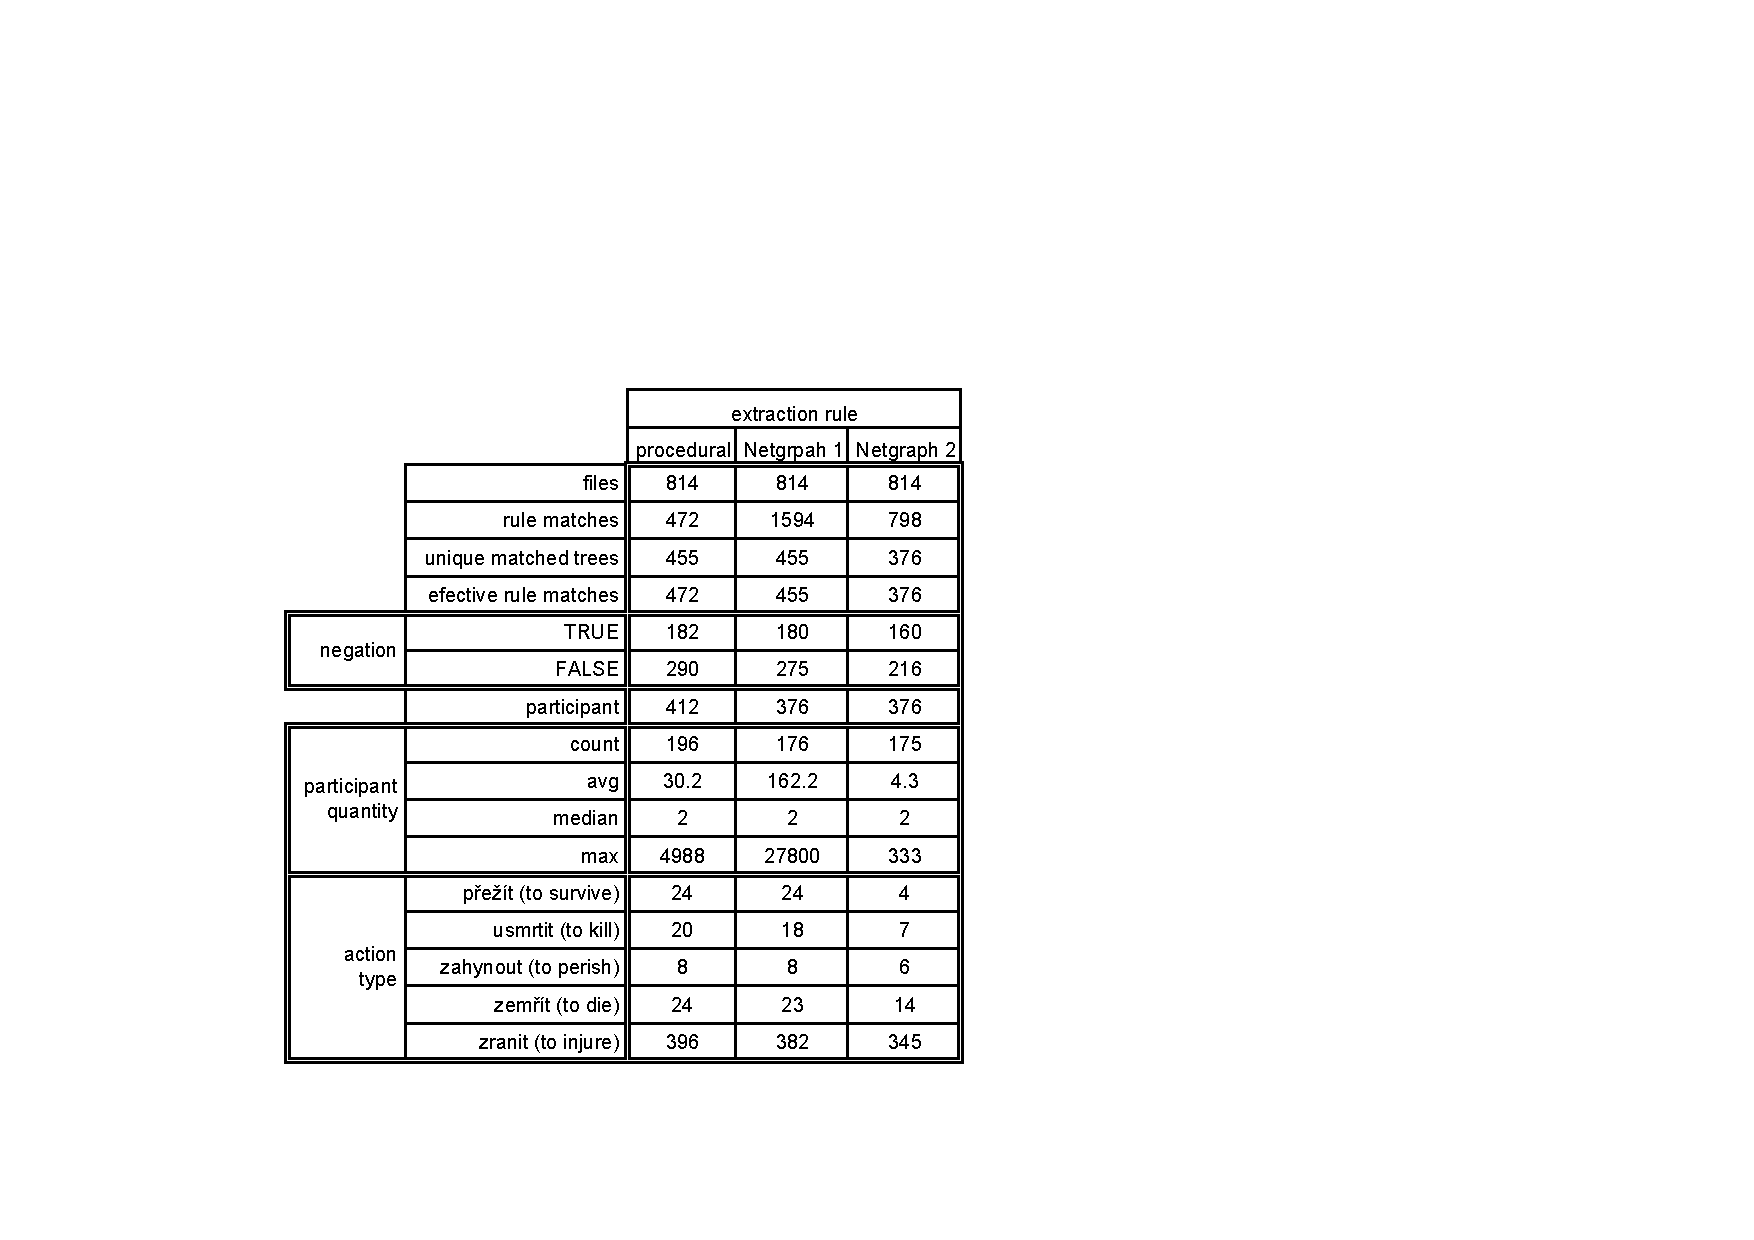
\includegraphics[angle=-90,width=0.6\hsize]{tab_manual_rules}
	\caption{Evaluation of manually created rules (bigger dataset without manual annotations).}
	\label{tab:ch50_tab_manual_rules}
\end{table}


\begin{description}
	\item[Files]
The same set of 814 files (texts) was used in all the experiments.

	\item[Rule matches]
The presence of optional nodes in a query increases the number of possibilities how a Netgraph query can be matched to a single linguistic tree. An optional node might or might not be marked in the result. The number of possible matches is also increased if there are more compatible nodes in a candidate tree that can be matched with a single query node. This can even be true for the participant query node (4) in the case of Netgraph based rules if a sentence mentions more than one affected person. This can be marked as a mistake in the rule design -- it does not count with such possibility, or it can be taken as a drawback of the current evaluation algorithm of the Netgraph based method -- it should put all the possibilities to the output. Note that this issue does not concern the procedural method, which outputs all the matching participants.

	\item[Unique matched trees]
This number represents the number of unique trees matched by the extraction rule.

	\item[Effective rule matches]
Because the procedural rules and the Netgraph based rules are evaluated in a different way, the way of selection of effective matches (matches that are used for the output) is also different. In the procedural case all matches are used because every such match is tied up with a different verb in a sentence. In this case more matches per sentence (tree) are only possible for complex sentences with more verbs and therefore every match is applicable because it is connected with a different piece of information.\\
In the Netgraph case it is necessary to select the most relevant matches of all possible ones. The first longest (maximum of optional nodes) match for each tree is selected. This is unfortunately not optimal and also not consistent with the procedural case, but it is the easiest option for the implementation (Netgraph can be directly used in that case.)

	\item[Negation, participant, participant quantity (count), action type]
These values represent numbers of matching nodes (or more precisely of pieces of extracted information) of the given type. For example values of participant are the numbers of all participants (node number 4 in the Netgraph based rule) identified by the extraction rule and values of \emph{p�e��t} (survive) are numbers of matching action type nodes with the value of \emph{p�e��t} (survive). Note that some postprocessing of the Netgraph based output was necessary to count TRUE and FLASE negation values.

	\item[Participant quantity]
Values in this group are all connected with the quantity kind of information. It expresses the quantity of participants involved in the corresponding incident action. This kind of information is numeric so some numerical calculations can be made (average value, median and maximum value). Again postprocessing of the Netgraph based output was necessary to obtain these values -- in this case translation of seven kinds of numerals to numbers (\emph{jeden} - 1, \emph{dva} - 2, \emph{t�i} - 3, \emph{�ty�i} - 4, \emph{�est} - 6, \emph{sedm} - 7, \emph{osm} - 8). Note that the vale of average is strongly affected by the very few high numbers present in the results (the values 1 and 2 accounted for more than half of the results.)\\
Values of participant quantity also demonstrate several errors made by the particular extraction rules, see bellow for details.
\end{description}





















\subsubsection{Detected errors}

Results of the extraction were investigated only partly; no formal evaluation is available in this case (except on a small evaluation set, see bellow: the second experiment). About 10-20\% of information was not extracted because of errors of linguistic parsing; majority of the errors was made in long complex sentences, which are known to be difficult for linguistic processing. There was only a few of false positives. A nice example can be traced from the maximum values of participant quantity in Table 99. Three different numbers were found in the three experiments: 27800, 4988 and 333. The number of 27800 is actually a number of chickens that died during one of the accidents. The number was extracted by the first Netgraph based rule because the query node 4 (participant) was marked as optional and omitted during the evaluation. This node normally ensures that the participant is one of: person, man, woman, child, driver, etc.
Numbers 4988 and 333 are both correct. They were both used in the same sentence, which summarized numbers of injured (4988) and killed (333) people during one whole year. Although the sentence was quite complex it was linguistically parsed correctly and also the procedural rule managed to extract both numbers correctly. The Netgraph based rule extracted only the first number in the sentence because the current evaluation algorithm does not allow multiple matches per sentence (see above the comments of rule matches and effective rule matches).


\subsection{Czech Fireman Qualitative}


\begin{table}
	\centering
	\begin{tabular}{|r|c|c|c|c|c|c|}
		\hline
		 & correct & missing & spurious & recall & precision & $F_1$\\
		\hline
		injuries & 3 & 29 & 0 & 0.09 & 1 & 0.17\\
		\hline
		fatalities & 1 & 10 & 0 & 0.09 & 1 & 0.17\\
		\hline
	\end{tabular}
	\caption{Evaluation of the manually created rule form Figure~\ref{fig:ch50_extract_patern} on the manually annotated dataset.}
	\label{tab:ch50_extract_patern_eval}
\end{table}



In the second experiment a manually annotated collection of 50 fireman news texts was used. Having the extraction rule from the previous experiment and a set of manually annotated texts it is only natural to ask a question about the success of the extraction rule on that collection. Table~\ref{tab:ch50_extract_patern_eval} summarizes the results. These results are far from satisfactory; the recall of 0.09 is something that is far from any acceptable use. Several explanations of the issue can be provided. The extraction rule serves more for a demonstration than for exhausting coverage of all possible cases. The extraction rule looks for particular verb (to injure, to die, etc.) but the information can be also expressed by an adjective (injured driver, death passenger, etc.); another extraction rules should be constructed for these and other cases. The training collection used for the design was also of a different spectrum of texts.



On the other hand this experiment shows how a manually annotated collection contributes to the quality of extraction rules. We can never know if the extraction rule is usable until a formal evaluated is made. Also the fact that the precision is strictly 1 should be noted. This means that the extraction rule made no mistake in those cases when it provided some output.



\subsubsection{Manual Design of Rules Using Training Data Set}  

\begin{table}
	\centering
	\begin{tabular}{|r|c|c|c|c|c|c|}
		\hline
		 & correct & missing & spurious & recall & precision & $F_1$\\
		\hline
		manual rules & 5 & 2 & 0 & 0.71 & 1 & 0.83\\
		\hline
		ILP rules & 5 & 2 & 0 & 0.71 & 1 & 0.83\\
		\hline
	\end{tabular}
	\caption{Evaluation of the manually created rules and ILP learned rules (manually annotated dataset was used for rule design (training half) and evaluation (testing half) -- see the description of the second experiment in text.)}
	\label{tab:ch50_damage_manual_eval}
\end{table}

\begin{table}
	\centering
	\begin{tabular}{|r|c|c|c|c|c|c|}
		\hline
		 & correct & missing & spurious & recall & precision & $F_1$\\
		\hline
		manual rules & 4 & 1 & 1 & 0.8 & 0.8 & 0.8\\
		\hline
		ILP rules & 4 & 1 & 1 & 0.8 & 0.8 & 0.8\\
		\hline
	\end{tabular}
	\caption{Cross method comparison of found instances.}
	\label{tab:ch50_damage_cross_method}
\end{table}




Next question that naturally emerges is: How would be the performance if the rules were designed with the support of a manually annotated collection? An additional experiment was made to answer that question. The collection was split into two even parts -- training part and testing part. A manually created rule was designed so that it correctly matched with all annotations of the training part and then it was evaluated on the testing part. For the validity of the experiment it was necessary that the designer did not have any knowledge about the data of the testing part; that is why we used a different extraction task (damage instead of injuries and fatalities).We have also compared the performance of the manually created rule with a rule learned by the ILP machine learning engine (see Chapter~\ref{ch:ILP_Learning}).

The results are summarized in Table~\ref{tab:ch50_damage_manual_eval}. Both kinds of rules (manually designed and learned by ILP) performed the same (recall: 0.71, precision: 1); both the methods correctly found 5 instances and they were both unable to find 2 instances. From the cross coverage comparison in 
Table~\ref{tab:ch50_damage_cross_method} it is apparent that the methods agreed on 4 instances and each method was able to discovered one instance that the other did not discover. Such results could be accepted for a practical application but we must not forget the fact that the collection is very small and only single evidence is provided by the experiment, so it dies not provide any statistical significance (getting statistically significant results would require experiments with different datasets, extraction tasks and human designers.) 



\section{Evaluation of Learned Rules}

\subsection{Czech Fireman Performance}

\subsection{Acquisitions Performance}

\subsection{?Acquisitions Time?}

\section{Evaluation of Shareable Extraction Ontologies Performance} \label{sec:eval_Shareable_Extraction_Ontologies}

\subsection{Reasoners}

\subsection{Czech Fireman Time}

\subsection{Acquisitions Time}

\section{Evaluation of Fuzzy ILP Classification}

\subsection{Czech Fireman Performance}

\subsection{UCI Performance}

\subsection{UCI Time}
